\chapter{Intelig{\^e}ncia Artificial}

\lipsum[1-2]

\section{Aprendizado de M{\'a}quina}

\lipsum[3-4]

\section{Aprendizado por reforco}

O Aprendizado de refor{\c c}o se trata se uma subcategoria de
aprendizado de m{\'a}quina que, de forma sumarizada, mapeia situa{\c
  c}{\~o}es a a{\c c}oes de forma a maximizar uma recompensa
num{\'e}rica. O aprendiz n{\~a}o {\'e} auxiliado em que a{\c c}{\~o}es
tomar, mas deve descobrir quais a{\c c}{\~o}es rendem mais recompensas
ao experiment{\'a}-las \cite{kaelbling1996}. Esse m{\'e}todo
explorat{\'o}rio faz contraste com m{\'e}todos de aprendizado
\textit{supervisionados}, em que o algoritmo recebe a informa{\c
  c}{\~a}o ``correta'' e tenta se aproximar ao m{\'a}ximo dessa
solu{\c c}{\~a}o conhecida; e tamb{\'e}m com os m{\'e}todos n{\~a}o
supervisionados, que utilizam m{\'e}todos de associa{\c c}{\~a}o e
\textit{clustering} para tomar suas decis{\~o}es. A
\autoref{fig_learnings} ilustra as rela{\c c}{\~o}es e principais
diferen{\c c}as entre esses m{\'e}todos.

\begin{figure}[htb]
  \centering
  \caption{\label{fig_learnings}Tabela com classifica{\c c}{\~o}es dos diferentes m{\'e}todos de aprendizado de m{\'a}quina.}
  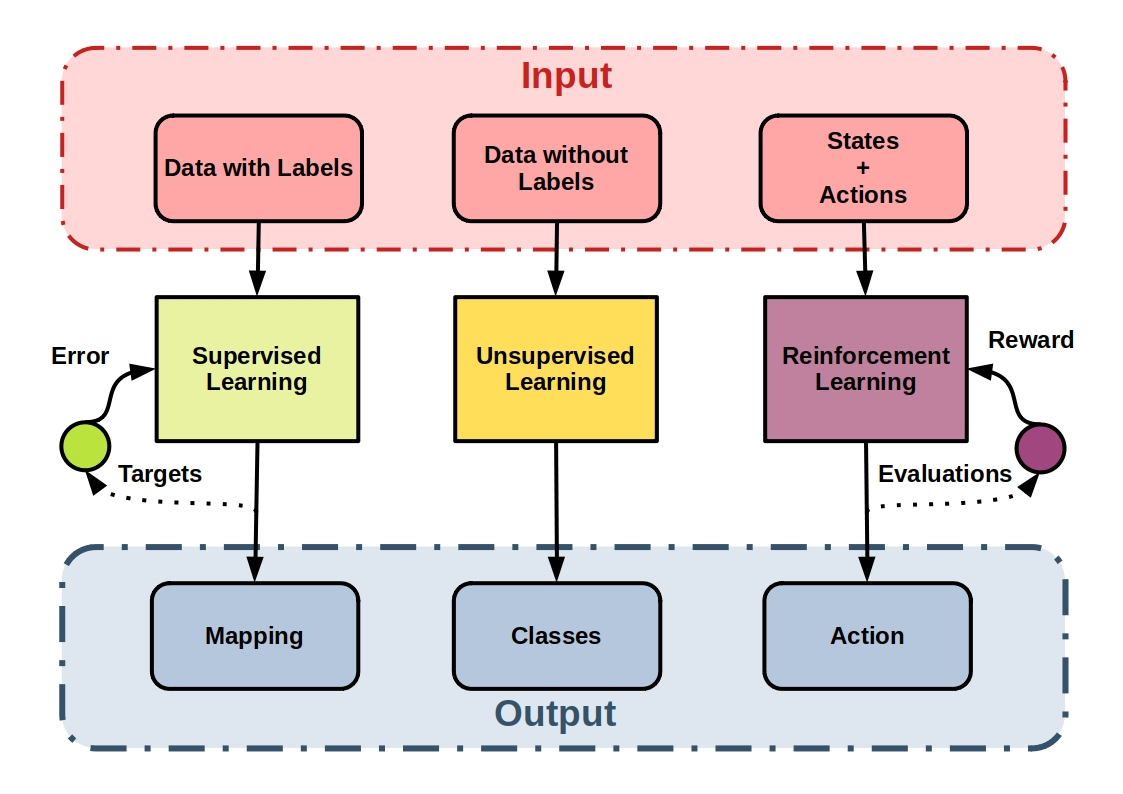
\includegraphics[width=0.7\textwidth]{images/unsupervised_supervised_reinforcement.jpeg}
  \legend{
    \protect\footnotemark
    Dispon{\'i}vel em: \url{https://starship-knowledge.com}. Acesso em: 4 Set. 2022.
  }
\end{figure}

\footnotetext{Imagem retirada de: \url{https://starship-knowledge.com/supervised-vs-unsupervised-vs-reinforcement}}


Esse tipo de aprendizado facilita ou at{\'e} possibilita experimentos
em que outros m{\'e}todos teriam muita dificuldade ou aumentariam a
complexidade do problema significativamente.
\citeonline{sutton2018reinforcement} indica que esse campo de estudo
tem atra{\'i}do cada vez mais interesse nas comunidades de IA e ML,
pelo seu modo de programar agentes por recompensas e puni{\c c}{\~o}es
atraves de tentativa e erro e sem precisar indicar \textit{como} o
problema deve ser resolvido.

Uma das principais aplica{\c c}{\~o}es de aprendizado por refor{\c c}o
se faz em problemas no espa{\c c}o f{\'i}sico, em que se recebe uma
quantidade grande de dados e que a rela{\c c}{\~a}o entre tais dados e
a a{\c c}{\~a}o ou resultado se faz dif{\'i}cil por meios
matem{\'a}ticos. Enquanto esses algor{\'i}tmos performam muito bem na
resolu{\c c}{\~a}o dos problemas, o processo de treinamento no mundo
real pode ser extremamente custoso e demorado. Nestes casos, simula{\c
  c}{\~o}es (contanto que sejam pr{\'o}ximas o suficiente da
realidade) podem trazer uma atraente alternativa para simplificar o
treinamento de um modelo complexo \cite{Rao_2020_CVPR}.

\section{NEAT}

\lipsum[6-8]
